Motion planning is needed for tensegrity robots to perform complex
tasks, such as goal-directed locomotion over uneven terrains.  Early
methods defined the desired trajectory for the structure's center of
mass \cite{Pinaud2003Path-Planning-f} or for some of its nodes
\cite{Wijdeven:2005dz} in the workspace.  Then, they divided the
trajectory into small segments, and for each of them, a stable
structure configuration was found using optimization.  But collisions
were not considered, which motivated approaches for (self-)collision
avoidance \cite{Xu2013Collision-free-, hernandez2009reconfigurable},
while keeping the structure stable. Recent path planning approaches
take collisions into account, but the control process is assumed slow
enough to eliminate any dynamic effects \cite{Xu2013Collision-free-,
Porta:2015aa}. This quasistatic assumption is often used in
tensegrity-based civil structures \cite{Rhode-Barbarigos:2012fv} but
is not easily justifiable in robotic applications.

\subsection{Efficient Kinodynamic Planning for Tensegrity Robots}

A tensegrity planner should be able to select a reconfiguration that
takes advantage of nonlinear dynamics to emulate behaviors, such as
running, jumping, and climbing, instead of limiting the structure to
slow reconfigurations. At the same time it should deal with the
high-dimensionality of a tensegrity robot's state space. Various
alternatives can be considered, as long as they can deal with
significant dynamics and complex contacts.

Trajectory planning can be formulated as a non-convex constraint
optimization, where a trajectory cost function must be minimized given
constraints arising from collision avoidance and actuator limits.  One
way to solve this problem is sequential convex optimization, where a
convex approximation around a trajectory is computed in an iterative
manner \cite{Schulman:2014aa}. This framework has shown promise in
dynamical systems \cite{Schulman:2014aa} and recently in soft
manipulators \cite{Marchese:2016aa}. At the same time, it does not
provide performance guarantees, as it may get stuck in local minima
where constraints are violated. Approaches, such as {\tt
CHOMP} \cite{Zucker:2013aa}, introduce a Monte Carlo process to
achieve probabilistic completeness. Nevertheless, there are many
implementation aspects that need to be addressed for such methods: a)
simplifications, such as approximating the robot geometry with spheres
may not be appropriate for tensegrities, b) and it may not be easy to
define certain primitives, such as Jacobians, or formulating complex
constraints.

An alternative that provides probabilistic completeness is founded on
sampling-based motion planning~\cite{Kavraki1996Probabilistic-R},
which finds valid robot configurations and connects them with locally
valid paths. Tree-based variants, such as {\tt
RRT}~\cite{LaValle2001}, can deal with significant dynamics as they
only need a forward propagation model, such as a physics engine, to
simulate the progression of a system's state.  Recently the conditions
under which these methods achieve asymptotic optimality have been
identified for kinematic systems
\cite{Karaman:2011aa}. Two recent developments also bring the hope
that sampling-based methods can provide global trajectories for
tensegrity robots in a computationally efficient manner, while
considering complex physical interactions:
\begin{myitem}
  \item[a)] efficient physics-based simulation for tensegrity robots,
    which are verified in hardware, are now available
    \cite{Caluwaerts2013rsif};
  \item[b)] asymptotically optimal and computationally efficient
    sampling-based planners have been developed for highly nonlinear,
    underactuated dynamics \cite{Li2015Sparse-Methods-}.
\end{myitem}

Fig.~\ref{fig:tens_example} illustrates a trajectory computed by such
a method \cite{Li2015Sparse-Methods-} for a simulated SUPERball
robot~\cite{SunSpiralSoftware}. The method provides anytime
properties, i.e., it returns trajectories of increasing quality as
computation time increases. The implementation behind
Fig.~\ref{fig:tens_example} randomly samples controls for the robot
and then optimizes over the resulting trajectories.

While promising, the above implementation is not taking advantage of
morphological computation as the planner reasons about the underlying
robot at its full complexity. One way to improve performance is the
integration of such high-level dynamical planners with lower-level
controllers, such as {\tt CPGs} \cite{Ijspeert2008,
Bliss2013Central-Pattern,MirletzSoftRobotics}. The latter take
advantage of morphological computation and provide identifiable motion
behaviors adaptable to different terrains. In such an integration, the
high-level planner can explore the space by sampling from a library of
maneuvers/behaviors by invoking different low-level controllers. This
can potentially provide a general framework for goal-directed
multi-modal locomotion of tensegrity structures that takes advantage
of morphological computation \cite{Nurzaman:2015aa,
Khazanov:2014aa}. It is useful to consider whether probabilistic
completeness and asymptotic optimality can still be provided for the
integrated framework.

\subsection{Re-Planning in Belief Space with Complex Dynamics}

Despite the progress in tensegrity modeling and even if dynamics are
reasonably taken into account, modeling errors and noise will result
in inaccurate execution of trajectories. One way to deal with this
issue is to represent uncertainty about the robot state as a
probability distribution, and plan in the set of distributions over
states, called the belief space. In this context, the planner aims to
compute the trajectory that maximizes the probability of success in
reaching a desired target. This challenge corresponds to a Partially
Observable Markov Decision Process ({\tt POMDP})
\cite{Kaebling:1998aa}. Planning in the belief space is challenging:
\begin{myitem}
\item[a)] A policy needs to be computed, where an action must be mapped
  to every possible belief distribution, which is a large, continuous
  space.
\item[b)] The resulting belief state dynamics are highly nonlinear
  and underactuated.
\end{myitem}
Nevertheless, recent advances have shown that motion planning in
belief space is becoming practical for many medium size problems by
employing reasonable approximations and efficient algorithmic tools
\cite{Platt:2010aa,Bai:2012aa}, bringing the
hope of potentially addressing more complex problems.

\begin{figure}[h!]
  \vspace{-.1in}
  \centering
\includegraphics[width=.48\textwidth]{figures/belief_replanning.png}
\vspace{-0.3in}
\caption{Replanning in belief space, where the first action of a plan
  is executed and the planner is called again given an updated
  belief. This allows the use of conformant planning, which operates
  in the belief space but does not compute a policy. Instead it
  returns the most robust trajectory.}\vspace{-0.1in}
\label{fig:belief_replanning}
\end{figure}

For instance, one way to reduce the complexity of the first challenge
above is to follow a replanning approach in belief space
\cite{Platt:2010aa}, similar to model predictive control, as
illustrated in Fig.~\ref{fig:belief_replanning}. In this case, only
the first action of the plan is executed and after the belief state is
updated, the planner is called again. This means that the planner does
not need to map actions to every possible belief but instead only
compute the most robust trajectory given the current initial belief,
the probabilistic transition model, and with no online observations.
This type of conformant planning, or a Non-Observable Markov Decision
Process, is easier than computing a general {\tt POMDP} policy.

Even after the consideration of a replanning approach, the second
challenge remains, i.e., the conformant planner needs to optimize the
robustness of trajectories in a highly nonlinear and underactuated
state space. Nevertheless, the recent sampling-based motion planners
for computing asymptotically optimal trajectories for complex
dynamical systems can now address such problems
\cite{Li2015Sparse-Methods-}. Recent work has shown that these methods
can be used for belief space conformant planning, where the objective
is to compute control inputs for high-dimensional, nonlinear and
underactuated systems that safely drive them to a goal region with a
probability above a given threshold \cite{Littlefield:2015aa}.

The representation of the underlying belief plays a critical role. The
high-dimensionality of tensegrities, the multi-modality from the
presence of contacts, and the highly nonlinear nature of the dynamics
pose significant challenges to both parametric representations, such
as Gaussian beliefs, and non-parametric ones, such as particle
filters. The highlighted recent work has followed a particle
representation, which can deal with multi-modality but is
computationally expensive. Figure \ref{fig:particles} shows the
propagation of multiple particles for the SUPERball given the same
control under the presence of noise.  It is interesting to consider
how to achieve effective belief space conformant replanning in the
case of tensegrity robots and focus on the proper modeling and fast
computation of the resulting uncertainty.

\begin{figure}[t]
\centering
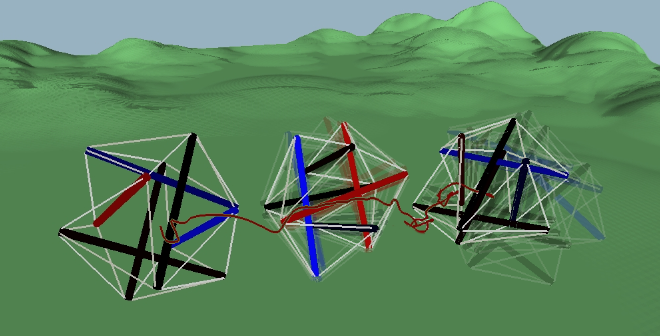
\includegraphics[width=.48\textwidth]{figures/particles.png}
\vspace{-0.3in}
\caption{A trajectory for the SUPERBall in belief space, where the
  application of controls can result in different outcomes due to noise.
  For the same control sequence a belief distribution over possible
  future states arises. A particle representation is followed for the
  belief \cite{Littlefield:2015aa}, which is illustrated as
  transparent versions of the robot.}  \vspace{-0.25in}
\label{fig:particles}
\end{figure}

\subsection {Model-based feedback motion planning}

Another avenue for dealing with noise and uncertainty involves the use
of feedback-based controllers, which aim to stabilize the robot at a
target state or trajectory, despite disturbances. For global motion
planning, this requires composing a sequence of low-level feedback
controllers, as shown in Fig.~\ref{fig:funnelcake}.
which \emph{funnel} the system toward a desired target in a way that
local minima are avoided~\cite{Burridge:1999aa, Conner:2006aa}.

One way to implement this principle is through the framework of
whole-body control via an operational space formulation
\cite{Khatib:1987aa,Sentis2005}. This involves the definition of
artificial potential fields for different tasks and their
prioritization, so that lower priority tasks are allowed to influence
the robot given only access to the null-space of higher priority
primitives. Tasks can include the avoidance of self-collisions,
reaching a desired configuration, and maintaining a desired posture.
The formulation of an Elastic Roadmap over operational spaces is done
by tiling the underlying state space with different, locally valid
controllers and specifying the transitions between them, while also
allowing for fast responses to sensory input \cite{Yang2010}. A
challenge for tensegrity robots is defining the artificial potential
fields in a way that they are valid for significant subsets of the
state space. Related to the challenge of defining proper Jacobians for
these systems, defining effective potential fields is not trivial.
Much like trajectory optimization methods, it is typically difficult
to argue about the properties and quality of paths generated from such
feedback controllers.

\begin{wrapfigure}{r}{0.2\textwidth}
  \centering
  \vspace{-.15in}
\includegraphics[width=.2\textwidth]{figures/Funnel.png}
\vspace{-0.2in}

\caption{The basic principle in feedback-based planning. The resulting
  state of a controller should be in the region of attraction of
  another.  The union of these regions should cover the state space so
  that the composition of controllers leads to the goal from any
  initial state.\vspace{-0.1in}}
\label{fig:funnelcake}
\end{wrapfigure}

An alternative methodology aims to provide probabilistic completeness
for feedback-based planning by composing multiple Linearized Quadratic
Regulators ({\tt LQR}), where each regulator stabilizes the system
around an individual trajectory. The composition can result in a
tree-like structure that allows for global planning
\cite{Tedrake2010}, where the {\tt LQR}-trees incrementally cover the
state space with their regions of attraction. A region of attraction
is the subset of the state space where the application of an {\tt LQR}
controller allows the stabilization of the system to a desired
trajectory.  Recent progress has allowed the conservative computation
of such areas for certain systems with dynamics.  A simulation-based
methodology has also been proposed that aims to approximate these
regions given access only to a simulator for the underlying system
\cite{Reist2010}. Applying this line of work on tensegrity robots can
potentially result in feedback solutions that can provide a certificate
of completeness.  It requires the formulation
of locally valid {\tt LQR} controllers for tensegrity robots with
computable regions of attractions, even if approximate. Such
controllers and regions of attractions should be generated quickly
given new sensor data.

The application of effective artificial potential fields or {\tt LQR}
controllers on tensegrity robots may prove difficult due to challenges in modeling  
complex dynamic interactions with the environment.  As pointed out in Section
\ref{sec:control}, however, effective low-level and model-free
locomotion controllers have already been defined for tensegrity
structures, such as those based on {\tt
CPG}s \cite{MirletzSoftRobotics, Caluwaerts2013rsif,
Bliss2013Central-Pattern}.  It is interesting to explore the
composition of such controllers in a way that global feedback-based
motion planning can be achieved. This will require exploration of the
conditions under which they work and how transitioning between
different controllers can be achieved, thereby synthesizing
certificates for whether a particular controller can achieve a desired
result. This direction also indicates one way that model-based
planning principles can be integrated with developments in the
model-free low-level controller domain.

\begin{comment}
\komment{

Given the development of effective controllers specifically for
tensegrity structures, such as {\tt CPG}s, one can focus on integrating
these controllers so as to solve more complex planning problems, while
providing feedback solutions with guarantees. This would require that
these controllers are able to provide some form of certificates about
their effectiveness, i.e., the conditions under which they work,
region of attraction, etc..}

\komment{Nice visuals can be generated for many of the principles
for the above set of methods.}
\end{comment}
